\subsection{Git}
\label{git}

Git is a so called \textit{distributed version control system}
\cite{git}, \cite{gitwiki} created by Linus Torvalds
\cite{gittalk} in order to help the development process of the
Linux operating system kernel, also created by Torvalds.
Since first conceived in 2005 \cite{gitbirth}, \textit{git} has become
one of the most used tools in modern software development today and
very many things can be said about how to effectively \textit{use}
git in order to organize source code versioning
and the whole collaborative software development process \cite{gitbook}.

Unfortunately the information about its interal structure and workings
is disproportionally rare compared to the massive amounts of tutorials
and usage guides. However, it is the combination of the internal
structure of git and its user interface that is of relevance to the
work presented here.
\newline

Since git was originally conceived to be a version control system
for source code and source code is most widely stored in files,
git operates on the file level and tracks changes to lines in files.
So from the user perspective, these are normal file system files
which are edited and stored just as any other files. Git does not
interfere with any operations of the underlying file system.
It is therefor completely invisible during the file editing
process.

After a change of a file has been saved (persisted to the underlying
file system) the user can issue git commands, e.g. using the
git command line tool, in order to instruct git to track and
\textit{note} these changes. In order to advance the git repository
to a new state, these changes need to be \textit{commited}. This
will create a new vertex in the history log of git and will advance
the current head pointer of the git repository to this new
version. It's important to note, that there is no fixed commit size.
Commits can contain any number of changes, even of different files.
It is up to the user to decide the \textit{distance} between
steps.

\begin{wrapfigure}{r}{0.5\textwidth}

  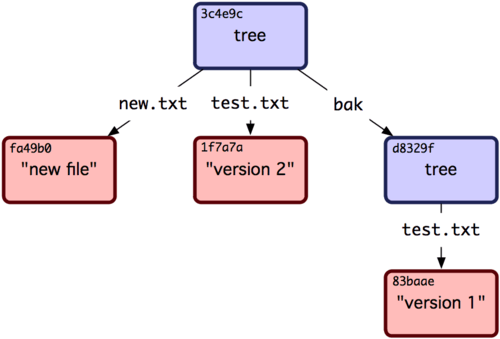
\includegraphics[width=0.5\textwidth]{git.png}
  \caption{Example of Git's internal tree structure based on content hashing.}
  \label{git}

\end{wrapfigure}

Git then stores the content of the tracked files as so called
\textit{blobs} and addresses them by the hash of their content.
Therefor behaving like a \textit{content addressable file system}
underneath. In order to store the file and directory structure
a tree structure is used in which blobs represent files and
subtrees represent directories, as shown in Fig.\ref{git} which
was taken from \cite{gitinternals}. It's important to note that
if a file is changed by the user and that file is then tracked
and the change committed to git, the hash of the content of the
file will be different compared to the earlier version of the file.
Therefor git will store the complete file again, now with its
new content and under the new hash. Only in later stages of the
repository will git use \textit{delta encoding and compression}
in order to eliminate duplicate content, i.e. when pushing to
a remote repository.
Keeping every single version of file identified by its content
hash is what allows git to be able to go back in time and fully
restore \textit{any} version of the repository ever committed.

This is all completely hidden from the user. From the user
perspective the file that she just changed, really changed.
Because git does not interfere with the underlying file system
a change in a file is persisted and permanent. It's the user
instructing git to take a \textit{content snapshot} of the current
state of the repository containing the content of all its files
and directories when issuing a commit command.

So the content snapshot becomes an immutable \textit{fact} and is
appended to the internal repository history. Just like a fact is
appended to the fact log that is Datomic, as introdudec in chapter
\ref{datomic}. But since the file really changes for the user,
she always immediately sees the latest state of the world but
has the possibility to check out earlier versions of the world.

Therefor the user interface is stateful. If a file is deleted
it's gone from the directory. But it is possible to recreate
the directory state in which it existed, including its content,
if a snapshot of that state was recorded. This means that it is
possible to change a file and then revert the change or to
create a file and then delete it again without git
ever noticing. The user has full control of the
history of the repository and needs to decide which intermediate
states of the repository become immutable facts by instructing
git to take a content snapshot. But since the changing of the
current files and also the recreation of earlier versions happen in
the extact same directory, the user experience feels more like working
in a stateful environment and persisting the current \textit{state}
down to the immutability layer. It feels like a stateful system
on top of an immutable system, instead of just dumping backups to
a data base.
\newline
So it is not necessary to stick to immutability all the way up
to the user interface in order to benefit from the advantages
of an immutable system because user actions aren't always final.
They don't always represent irreversible facts that should always
stay true. As I would like to argue, most people iterate when
working. They have an idea that seems plausible, implement that
idea and then realize that they haven't thought of this and that,
or something else doesn't work out as planned. So they change,
adjust and iterate until a satisfying solution is found or the
necessary resources for doing so have run out. Which is exactly
what is best represented by a stateful environment.

But there will be intermediate steps that seem significant, and
these can be recorded as immutable facts in order to allow for backtracking
or to serve as documentation or as cached results for other work in progress
that somehow arrives at the same intermediate result.



